\section{مقدمه و تعاریف پایه}

% Slide 1: Title Slide
\begin{frame}[plain]
\titlepage
\end{frame}

% Slide 2: Outline
\begin{frame}{سرفصل مطالب}{\lr{Outline}}
\begin{itemize}\setlength{\itemsep}{8pt}
    \item \textbf{تحلیل وابستگی چیست؟} \lr{(What is Association Analysis?)}
    \item \textbf{تولید مجموعه‌های اقلام مکرر} \lr{(Frequent Itemset Generation)}
    \item \textbf{تولید قواعد وابستگی} \lr{(Rule Generation)}
    \item \textbf{پیاده‌سازی در پایتون و معیارهای جذابیت} \lr{(Interestingness Measures)}
    \item \textbf{مدیریت ویژگی‌های پیوسته و دسته‌ای} \lr{(Continuous \& Categorical Attributes)}
    \item \textbf{کشف زیرگروه‌ها} \lr{(Subgroup Discovery)}
\end{itemize}
\end{frame}

% Slide 3: Motivation / Association Analysis
\begin{frame}{تحلیل وابستگی}{\lr{Association Analysis}}
\begin{columns}[T,onlytextwidth]
\begin{column}{0.65\textwidth}
\begin{itemize}\setlength{\itemsep}{6pt}
    \item \textbf{توسعهٔ نخستین الگوریتم‌ها} در اوایل دههٔ ۱۹۹۰ میلادی در شرکت \lr{IBM} توسط آگراوال و سریکانت \lr{(Agrawal \& Srikant)}.
    \item \textbf{انگیزهٔ اولیه:}
    \begin{itemize}\setlength{\itemsep}{3pt}
        \item دردسترس قرار گرفتن صندوق‌های فروشگاهی بارکددار
        \item \lr{(Availability of barcode cash registers)}
    \end{itemize}
\end{itemize}

\vspace{0.15cm}
\begin{center}
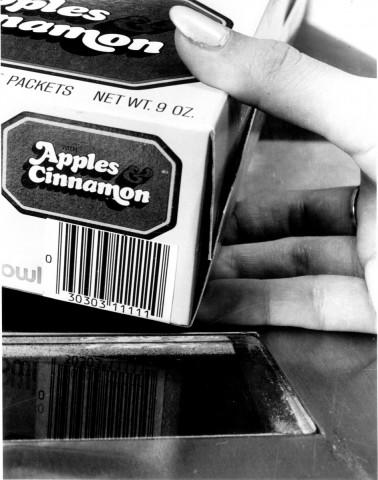
\includegraphics[height=2.4cm,keepaspectratio]{images/slide03_barcode_clean.jpeg}
\end{center}
\end{column}%
\begin{column}{0.32\textwidth}
\centering
\vspace{0.1cm}
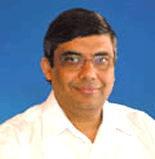
\includegraphics[width=0.58\linewidth,keepaspectratio]{images/slide03_agrawal_clean.png}\\[2pt]
{\scriptsize\lr{R. Agrawal}}

\vspace{0.35cm}
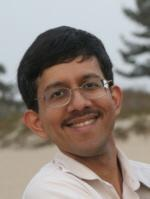
\includegraphics[width=0.58\linewidth,keepaspectratio]{images/slide03_srikant_clean.jpeg}\\[2pt]
{\scriptsize\lr{R. Srikant}}
\end{column}
\end{columns}
\end{frame}

% Slide 4: Scope and Application Domains
\begin{frame}{تحلیل وابستگی}{\lr{Association Analysis}}
\begin{itemize}\setlength{\itemsep}{7pt}
    \item \textbf{در ابتدا برای «تحلیل سبد خرید» \lr{(Market Basket Analysis)} به کار رفت:}
    \begin{itemize}\setlength{\itemsep}{3pt}
        \item یافتن نحوهٔ ارتباط و وابستگی اقلام خریداری‌شده توسط مشتریان فروشگاه‌ها
    \end{itemize}
    \item \textbf{سپس به ساختارهای داده‌ای پیچیده‌تر گسترش یافت:}
    \begin{itemize}\setlength{\itemsep}{3pt}
        \item الگوهای ترتیبی \lr{(Sequential patterns)}
        \item الگوهای زیرگراف \lr{(Subgraph patterns)}
    \end{itemize}
    \item \textbf{و در سایر حوزه‌های کاربردی مورد استفاده قرار گرفت:}
    \begin{itemize}\setlength{\itemsep}{3pt}
        \item علوم زیستی و بیوانفورماتیک \lr{(Life science)}
        \item علوم اجتماعی \lr{(Social science)}
        \item کاوش کاربرد وب \lr{(Web usage mining)}
    \end{itemize}
\end{itemize}
\end{frame}

% Slide 5: Simple Approaches - Pearson Correlation
\begin{frame}{رویکردهای ساده}{\lr{Simple Approaches}}
\begin{itemize}\setlength{\itemsep}{4pt}
    \item برای فهمیدن اینکه آیا دو قلم کالا ($x$ و $y$) معمولاً \textbf{با هم خریده می‌شوند} یا خیر، می‌توانیم همبستگی آن‌ها را محاسبه کنیم.
    \item برای مثال، ضریب همبستگی پیرسون \lr{(Pearson's correlation coefficient - PCC)}:
    \begin{center}
    \begin{latin}
    \[
    \text{PCC} = \frac{\sum_{i=1}^n (p_i - \bar{p}) \cdot (a_i - \bar{a})}{\sqrt{\sum_{i=1}^n (p_i - \bar{p})^2} \cdot \sqrt{\sum_{i=1}^n (a_i - \bar{a})^2}}
    \]
    \end{latin}
    \end{center}
    \begin{itemize}\footnotesize\setlength{\itemsep}{1pt}
        \item $p_i$: مقدار پیش‌بینی‌شده \lr{(predicted value)}
        \item $a_i$: مقدار واقعی \lr{(actual value)}
    \end{itemize}
    \item \textbf{کدگذاری عددی \lr{(Numerical coding)}:}
    \begin{itemize}\footnotesize\setlength{\itemsep}{1pt}
        \item $1$: قلم کالا خریده شده است \lr{(item was bought)}
        \item $0$: قلم کالا خریده نشده است \lr{(item was not bought)}
    \end{itemize}
    \item $\bar{p}$ میانگین $p$ است (یعنی اینکه قلم کالای $x$ هر چند وقت یک‌بار خریده شده است).
\end{itemize}
\end{frame}

% Slide 6: Correlation Analysis in Python
\begin{frame}[fragile]{تحلیل همبستگی در پایتون}{\lr{Correlation Analysis in Python}}
\begin{itemize}\setlength{\itemsep}{2pt}
    \item به عنوان نمونه با استفاده از کتابخانهٔ پایتون \lr{Pandas}:
\end{itemize}
\vspace{-0.1cm}
\begin{center}
\begin{tcolorbox}[colback=black!5,colframe=black!25,arc=3pt,width=0.68\textwidth,left=6pt,right=6pt,top=2pt,bottom=2pt]
\begin{latin}
\fontsize{8}{10}\selectfont\ttfamily
import seaborn as sns\\
corr = dataframe.corr()\\
sns.heatmap(corr)
\end{latin}
\end{tcolorbox}
\end{center}
\vspace{-0.15cm}
\begin{center}
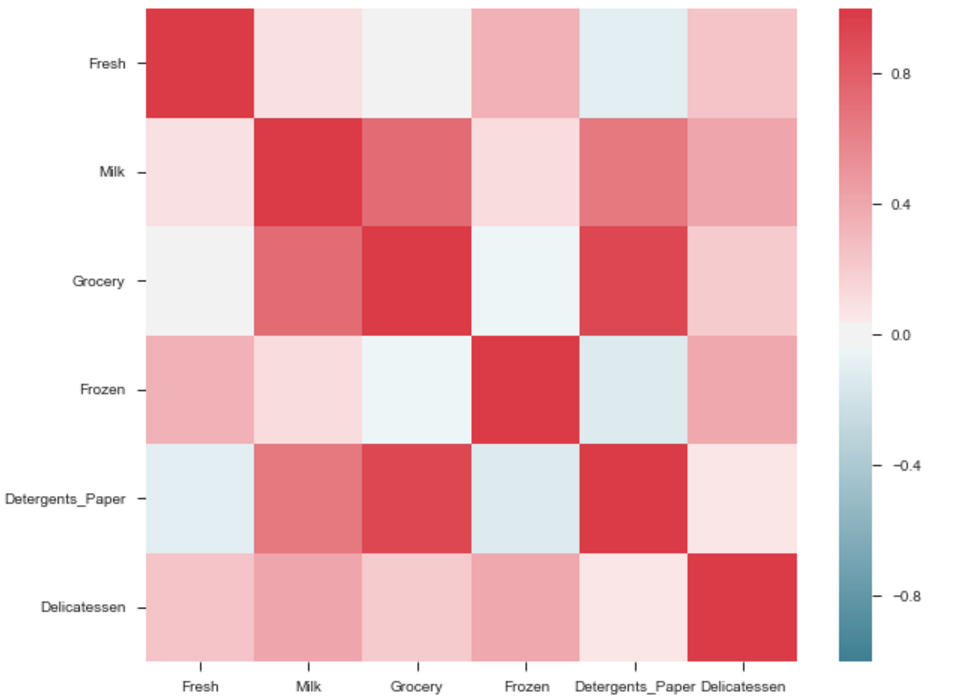
\includegraphics[height=3.4cm,keepaspectratio]{images/slide06_heatmap.png}
\end{center}
\end{frame}

% Slide 7: Problem Definition
\begin{frame}{تعریف مسئله}{\lr{Association Analysis: Problem Definition}}
\begin{columns}[T,onlytextwidth]
\begin{column}{0.58\textwidth}
\begin{itemize}\setlength{\itemsep}{5pt}
    \item با داشتن مجموعه‌ای از تراکنش‌ها، هدف \textbf{یافتن قواعدی} است که رخداد یک قلم کالا را بر پایه رخداد سایر اقلام در همان تراکنش پیش‌بینی نماید.
    \item \textbf{نمونه‌هایی از قواعد وابستگی:}
    \begin{center}
    \begin{latin}
    \small
    $\{\text{Diaper}\} \to \{\text{Beer}\}$ \\[2pt]
    $\{\text{Beer}, \text{Bread}\} \to \{\text{Milk}\}$ \\[2pt]
    $\{\text{Milk}, \text{Bread}\} \to \{\text{Eggs}, \text{Coke}\}$
    \end{latin}
    \end{center}
\end{itemize}

\vspace{0.15cm}
\begin{tcolorbox}[colback=mannheimblue!8,colframe=mannheimblue,arc=2pt,left=4pt,right=4pt,top=4pt,bottom=4pt]
\centering
\small \textbf{نکته مهم:} علامت استلزام ($\to$) بیانگر \textbf{«هم‌رخدادی»} است، نه رابطهٔ «علّیت»!\\[1pt]
{\scriptsize\lr{(Implication denotes co-occurrence, not causality!)}}
\end{tcolorbox}
\end{column}%
\begin{column}{0.40\textwidth}
\centering
\textbf{\small تراکنش‌های خرید}\\[1pt]
{\scriptsize\lr{(Shopping Transactions)}}\\[3pt]
\begin{latin}
\fontsize{7.5}{9.5}\selectfont
\begin{tabular}{|c|l|}
\hline
\rowcolor{mannheimblue!15}
\textbf{TID} & \textbf{Items} \\ \hline
1 & Bread, Milk \\ \hline
2 & Bread, Diaper, Beer, Eggs \\ \hline
3 & Milk, Diaper, Beer, Coke \\ \hline
4 & Bread, Milk, Diaper, Beer \\ \hline
5 & Bread, Milk, Diaper, Coke \\ \hline
\end{tabular}
\end{latin}
\end{column}
\end{columns}
\end{frame}

% Slide 8: Definition: Frequent Itemset
\begin{frame}{تعریف: مجموعه‌آیتم مکرر}{\lr{Definition: Frequent Itemset}}
\begin{columns}[T,onlytextwidth]
\begin{column}{0.58\textwidth}
\begin{itemize}\setlength{\itemsep}{3pt}\small
    \item \textbf{مجموعه‌آیتم} \lr{(Itemset)}
    \begin{itemize}\footnotesize
        \item مجموعه‌ای شامل یک یا چند قلم کالا (آیتم).
        \item مثال: \lr{\{Milk, Bread, Diaper\}}
        \item \textbf{$k$‌ـ‌مجموعه‌آیتم:} مجموعه‌آیتمی شامل $k$ قلم کالا.
    \end{itemize}
    \item \textbf{شمارش پشتیبان} \lr{(Support count, $\sigma$)}
    \begin{itemize}\footnotesize
        \item فراوانی رخداد یک مجموعه‌آیتم در کل داده‌ها:
        \par\vspace{1pt}\noindent\makebox[\linewidth][c]{$\displaystyle \sigma(\{\text{\lr{Milk, Bread, Diaper}}\}) = 2$}\par\vspace{1pt}
    \end{itemize}
    \item \textbf{پشتیبان} \lr{(Support, $s$)}
    \begin{itemize}\footnotesize
        \item کسر تراکنش‌های دربرگیرندهٔ مجموعه‌آیتم:
        \par\vspace{1pt}\noindent\makebox[\linewidth][c]{$\displaystyle s(\{\text{\lr{Milk, Bread, Diaper}}\}) = 2/5 = 0.4$}\par\vspace{1pt}
    \end{itemize}
    \item \textbf{مجموعه‌آیتم مکرر} \lr{(Frequent Itemset)}
    \begin{itemize}\footnotesize
        \item مجموعه‌آیتمی که پشتیبان آن $\ge \text{minsup}$ باشد.
    \end{itemize}
\end{itemize}
\end{column}%
\begin{column}{0.38\textwidth}
\centering
\textbf{\small تراکنش‌های خرید}\\[1pt]
{\scriptsize\lr{(Shopping Transactions)}}\\[3pt]
\begin{latin}
\fontsize{7.5}{9.5}\selectfont
\begin{tabular}{|c|l|}
\hline
\rowcolor{mannheimblue!15}
\textbf{TID} & \textbf{Items} \\ \hline
1 & Bread, Milk \\ \hline
2 & Bread, Diaper, Beer, Eggs \\ \hline
3 & Milk, Diaper, Beer, Coke \\ \hline
4 & Bread, Milk, Diaper, Beer \\ \hline
5 & Bread, Milk, Diaper, Coke \\ \hline
\end{tabular}
\end{latin}
\end{column}
\end{columns}
\end{frame}

% Slide 9: Definition: Association Rule
\begin{frame}{تعریف: قاعدهٔ وابستگی}{\lr{Definition: Association Rule}}
\begin{columns}[T,onlytextwidth]
\begin{column}{0.58\textwidth}
\begin{itemize}\setlength{\itemsep}{6pt}
    \item \textbf{قاعدهٔ وابستگی}: \lr{(Association Rule)}
    \begin{itemize}\setlength{\itemsep}{3pt}
        \item یک رابطه به فرم استلزام $X \to Y$ است که در آن $X$ و $Y$ دو مجموعه‌آیتم مجزا هستند: $X \cap Y = \emptyset$.
        \item \textbf{تفسیر:} هرگاه $X$ رخ دهد، $Y$ نیز با یک احتمال مشخص رخ خواهد داد.
    \end{itemize}
    \vspace{0.2cm}
    \item \textbf{بیان دقیق‌تر به صورت احتمال شرطی:}
    \begin{itemize}\setlength{\itemsep}{3pt}
        \item $P(Y \mid X)$: با فرض رخداد $X$، احتمال رخ دادن $Y$ چقدر است؟
    \end{itemize}
\end{itemize}
\end{column}%
\begin{column}{0.38\textwidth}
\centering
\textbf{\small تراکنش‌های خرید}\\[1pt]
{\scriptsize\lr{(Shopping Transactions)}}\\[3pt]
\begin{latin}
\fontsize{7.5}{9.5}\selectfont
\begin{tabular}{|c|l|}
\hline
\rowcolor{mannheimblue!15}
\textbf{TID} & \textbf{Items} \\ \hline
1 & Bread, Milk \\ \hline
2 & Bread, Diaper, Beer, Eggs \\ \hline
3 & Milk, Diaper, Beer, Coke \\ \hline
4 & Bread, Milk, Diaper, Beer \\ \hline
5 & Bread, Milk, Diaper, Coke \\ \hline
\end{tabular}
\end{latin}
\end{column}
\end{columns}
\end{frame}

% Slide 10: Rule Evaluation Example
\begin{frame}{ارزیابی قاعدهٔ وابستگی}{\lr{Definition: Association Rule}}
\begin{columns}[T,onlytextwidth]
\begin{column}{0.58\textwidth}
\begin{itemize}\setlength{\itemsep}{2pt}\small
    \item \textbf{مثال از قاعدهٔ وابستگی:}
    \begin{center}
    \begin{latin}
    $\underbrace{\{\text{\color{red}Milk, Diaper}\}}_{\text{\rl{مقدم / شرط}}} \to \underbrace{\{\text{\color{blue}Beer}\}}_{\text{\rl{مؤخر / نتیجه}}}$
    \end{latin}
    \end{center}
    \item \textbf{معیارهای ارزیابی قاعده:}
    \begin{itemize}\footnotesize
        \item \textbf{پشتیبان ($s$):} کسر تراکنش‌های دربرگیرندهٔ هر دو مجموعهٔ $X$ و $Y$ به صورت زیر است:
        \par\vspace{1pt}\noindent\makebox[\linewidth][c]{$\displaystyle s(X \to Y) = \frac{\sigma(X \cup Y)}{|T|} = \frac{2}{5} = 0.4$}\par\vspace{1pt}
        \item \textbf{اطمینان ($c$):} بسامد رخداد اقلام $Y$ در تراکنش‌های حاوی $X$ به این صورت محاسبه می‌شود:
        \par\vspace{1pt}\noindent\makebox[\linewidth][c]{$\displaystyle c(X \to Y) = \frac{\sigma(X \cup Y)}{\sigma(X)} = \frac{2}{3} \approx 0.67$}\par\vspace{1pt}
    \end{itemize}
\end{itemize}
\end{column}%
\begin{column}{0.38\textwidth}
\centering
\textbf{\small تراکنش‌های خرید}\\[1pt]
{\scriptsize\lr{(Shopping Transactions)}}\\[3pt]
\begin{latin}
\fontsize{7.5}{9.5}\selectfont
\begin{tabular}{|c|l|}
\hline
\rowcolor{mannheimblue!15}
\textbf{TID} & \textbf{Items} \\ \hline
1 & Bread, Milk \\ \hline
2 & Bread, Diaper, Beer, Eggs \\ \hline
3 & \textbf{\color{red}Milk}, \textbf{\color{red}Diaper}, \textbf{\color{blue}Beer}, Coke \\ \hline
4 & Bread, \textbf{\color{red}Milk}, \textbf{\color{red}Diaper}, \textbf{\color{blue}Beer} \\ \hline
5 & Bread, Milk, Diaper, Coke \\ \hline
\end{tabular}
\end{latin}
\end{column}
\end{columns}
\end{frame}

% Slide 11: The Association Rule Mining Task
\begin{frame}{مسئلهٔ کاوش قواعد وابستگی}{\lr{The Association Rule Mining Task}}
\begin{itemize}\setlength{\itemsep}{5pt}
    \item با داشتن مجموعه‌ای از تراکنش‌ها $T$، هدف کاوش قواعد وابستگی عبارت است از:
    \begin{center}
    \textbf{\large یافتن تمامی قواعدی که در دو شرط زیر صدق کنند:}
    \end{center}
    \begin{center}
    \begin{latin}
    $\text{support} \ge \text{minsup} \quad \text{and} \quad \text{confidence} \ge \text{minconf}$
    \end{latin}
    \end{center}
    \item دو آستانهٔ \lr{minsup} و \lr{minconf} توسط کاربر تعیین می‌شوند.
    \item \textbf{رویکرد جستجوی جامع} \lr{(Brute Force)}:
    \begin{itemize}\setlength{\itemsep}{2pt}
        \item فهرست کردن تمامی قواعد وابستگی ممکن در فضای مسئله
        \item محاسبهٔ مقدار پشتیبان و اطمینان برای تک‌تک قواعد
        \item حذف قواعدی که در آستانه‌های \lr{minsup} یا \lr{minconf} صدق نمی‌کنند.
    \end{itemize}
    \item \alert{\textbf{$\Rightarrow$ به دلیل تعداد عظیم نامزدها، جستجوی جامع از نظر محاسباتی غیرممکن است!}}
\end{itemize}
\end{frame}

% Slide 12: Mining Association Rules
\begin{frame}{استخراج قواعد وابستگی}{\lr{Mining Association Rules}}
\begin{columns}[T,onlytextwidth]
\begin{column}{0.58\textwidth}
\textbf{\small نمونه قواعد مستخرج:}
\begin{latin}
\footnotesize
\begin{itemize}\setlength{\itemsep}{1pt}
    \item $\{\text{Milk, Diaper}\} \to \{\text{Beer}\} \quad (s=0.4, c=0.67)$
    \item $\{\text{Milk, Beer}\} \to \{\text{Diaper}\} \quad (s=0.4, c=1.0)$
    \item $\{\text{Diaper, Beer}\} \to \{\text{Milk}\} \quad (s=0.4, c=0.67)$
    \item $\{\text{Beer}\} \to \{\text{Milk, Diaper}\} \quad (s=0.4, c=0.67)$
    \item $\{\text{Diaper}\} \to \{\text{Milk, Beer}\} \quad (s=0.4, c=0.5)$
    \item $\{\text{Milk}\} \to \{\text{Diaper, Beer}\} \quad (s=0.4, c=0.5)$
\end{itemize}
\end{latin}

\vspace{0.1cm}
\textbf{\small مشاهدات کلیدی:}
\begin{itemize}\footnotesize\setlength{\itemsep}{2pt}
    \item تمامی قواعد بالا افرازهای دودویی از یک مجموعه‌آیتم یکسان هستند: \lr{\{Milk, Diaper, Beer\}}.
    \item قواعد برگرفته از یک مجموعه‌آیتم یکسان، دارای \textbf{پشتیبان یکسان $s$} هستند؛ اما می‌توانند \textbf{اطمینان $c$ متفاوتی} داشته باشند.
    \item \alert{\textbf{نتیجه:}} می‌توانیم نیازمندی‌های پشتیبان و اطمینان را \textbf{از یکدیگر تفکیک} نماییم!
\end{itemize}
\end{column}%
\begin{column}{0.38\textwidth}
\centering
\textbf{\small تراکنش‌های خرید}\\[1pt]
{\scriptsize\lr{(Shopping Transactions)}}\\[3pt]
\begin{latin}
\fontsize{7.5}{9.5}\selectfont
\begin{tabular}{|c|l|}
\hline
\rowcolor{mannheimblue!15}
\textbf{TID} & \textbf{Items} \\ \hline
1 & Bread, Milk \\ \hline
2 & Bread, Diaper, Beer, Eggs \\ \hline
3 & Milk, Diaper, Beer, Coke \\ \hline
4 & Bread, Milk, Diaper, Beer \\ \hline
5 & Bread, Milk, Diaper, Coke \\ \hline
\end{tabular}

\vspace{0.3cm}
\[
s(X \to Y) = \frac{\sigma(X \cup Y)}{|T|}
\]
\end{latin}
\end{column}
\end{columns}
\end{frame}
